\documentclass[twoside]{book}

% Packages required by doxygen
\usepackage{fixltx2e}
\usepackage{calc}
\usepackage{doxygen}
\usepackage[export]{adjustbox} % also loads graphicx
\usepackage{graphicx}
\usepackage[utf8]{inputenc}
\usepackage{makeidx}
\usepackage{multicol}
\usepackage{multirow}
\PassOptionsToPackage{warn}{textcomp}
\usepackage{textcomp}
\usepackage[nointegrals]{wasysym}
\usepackage[table]{xcolor}

% Font selection
\usepackage[T1]{fontenc}
\usepackage[scaled=.90]{helvet}
\usepackage{courier}
\usepackage{amssymb}
\usepackage{sectsty}
\renewcommand{\familydefault}{\sfdefault}
\allsectionsfont{%
  \fontseries{bc}\selectfont%
  \color{darkgray}%
}
\renewcommand{\DoxyLabelFont}{%
  \fontseries{bc}\selectfont%
  \color{darkgray}%
}
\newcommand{\+}{\discretionary{\mbox{\scriptsize$\hookleftarrow$}}{}{}}

% Page & text layout
\usepackage{geometry}
\geometry{%
  a4paper,%
  top=2.5cm,%
  bottom=2.5cm,%
  left=2.5cm,%
  right=2.5cm%
}
\tolerance=750
\hfuzz=15pt
\hbadness=750
\setlength{\emergencystretch}{15pt}
\setlength{\parindent}{0cm}
\setlength{\parskip}{3ex plus 2ex minus 2ex}
\makeatletter
\renewcommand{\paragraph}{%
  \@startsection{paragraph}{4}{0ex}{-1.0ex}{1.0ex}{%
    \normalfont\normalsize\bfseries\SS@parafont%
  }%
}
\renewcommand{\subparagraph}{%
  \@startsection{subparagraph}{5}{0ex}{-1.0ex}{1.0ex}{%
    \normalfont\normalsize\bfseries\SS@subparafont%
  }%
}
\makeatother

% Headers & footers
\usepackage{fancyhdr}
\pagestyle{fancyplain}
\fancyhead[LE]{\fancyplain{}{\bfseries\thepage}}
\fancyhead[CE]{\fancyplain{}{}}
\fancyhead[RE]{\fancyplain{}{\bfseries\leftmark}}
\fancyhead[LO]{\fancyplain{}{\bfseries\rightmark}}
\fancyhead[CO]{\fancyplain{}{}}
\fancyhead[RO]{\fancyplain{}{\bfseries\thepage}}
\fancyfoot[LE]{\fancyplain{}{}}
\fancyfoot[CE]{\fancyplain{}{}}
\fancyfoot[RE]{\fancyplain{}{\bfseries\scriptsize Generated by Doxygen }}
\fancyfoot[LO]{\fancyplain{}{\bfseries\scriptsize Generated by Doxygen }}
\fancyfoot[CO]{\fancyplain{}{}}
\fancyfoot[RO]{\fancyplain{}{}}
\renewcommand{\footrulewidth}{0.4pt}
\renewcommand{\chaptermark}[1]{%
  \markboth{#1}{}%
}
\renewcommand{\sectionmark}[1]{%
  \markright{\thesection\ #1}%
}

% Indices & bibliography
\usepackage{natbib}
\usepackage[titles]{tocloft}
\setcounter{tocdepth}{3}
\setcounter{secnumdepth}{5}
\makeindex

% Hyperlinks (required, but should be loaded last)
\usepackage{ifpdf}
\ifpdf
  \usepackage[pdftex,pagebackref=true]{hyperref}
\else
  \usepackage[ps2pdf,pagebackref=true]{hyperref}
\fi
\hypersetup{%
  colorlinks=true,%
  linkcolor=blue,%
  citecolor=blue,%
  unicode%
}

% Custom commands
\newcommand{\clearemptydoublepage}{%
  \newpage{\pagestyle{empty}\cleardoublepage}%
}

\usepackage{caption}
\captionsetup{labelsep=space,justification=centering,font={bf},singlelinecheck=off,skip=4pt,position=top}

%===== C O N T E N T S =====

\begin{document}

% Titlepage & ToC
\hypersetup{pageanchor=false,
             bookmarksnumbered=true,
             pdfencoding=unicode
            }
\pagenumbering{alph}
\begin{titlepage}
\vspace*{7cm}
\begin{center}%
{\Large My Project }\\
\vspace*{1cm}
{\large Generated by Doxygen 1.8.15}\\
\end{center}
\end{titlepage}
\clearemptydoublepage
\pagenumbering{roman}
\tableofcontents
\clearemptydoublepage
\pagenumbering{arabic}
\hypersetup{pageanchor=true}

%--- Begin generated contents ---
\chapter{Hierarchical Index}
\section{Class Hierarchy}
This inheritance list is sorted roughly, but not completely, alphabetically\+:\begin{DoxyCompactList}
\item \contentsline{section}{circulo}{\pageref{classcirculo}}{}
\item \contentsline{section}{cubo}{\pageref{classcubo}}{}
\item \contentsline{section}{esfera}{\pageref{classesfera}}{}
\item \contentsline{section}{geometria}{\pageref{classgeometria}}{}
\item \contentsline{section}{paralelepipedo}{\pageref{classparalelepipedo}}{}
\item \contentsline{section}{piramide}{\pageref{classpiramide}}{}
\item \contentsline{section}{quadrado}{\pageref{classquadrado}}{}
\item \contentsline{section}{retangulo}{\pageref{classretangulo}}{}
\item \contentsline{section}{triangulo}{\pageref{classtriangulo}}{}
\item exception\begin{DoxyCompactList}
\item \contentsline{section}{Argumentos\+Errados}{\pageref{classArgumentosErrados}}{}
\item \contentsline{section}{Figura\+Nao\+Cadastrada}{\pageref{classFiguraNaoCadastrada}}{}
\item \contentsline{section}{Number}{\pageref{classNumber}}{}
\end{DoxyCompactList}
\end{DoxyCompactList}

\chapter{Class Index}
\section{Class List}
Here are the classes, structs, unions and interfaces with brief descriptions\+:\begin{DoxyCompactList}
\item\contentsline{section}{\mbox{\hyperlink{classbanco}{banco}} }{\pageref{classbanco}}{}
\item\contentsline{section}{\mbox{\hyperlink{classconta}{conta}} }{\pageref{classconta}}{}
\item\contentsline{section}{\mbox{\hyperlink{classcontaCorrente}{conta\+Corrente}} }{\pageref{classcontaCorrente}}{}
\item\contentsline{section}{\mbox{\hyperlink{classcontaPoupanca}{conta\+Poupanca}} }{\pageref{classcontaPoupanca}}{}
\item\contentsline{section}{\mbox{\hyperlink{classmovimentacao}{movimentacao}} }{\pageref{classmovimentacao}}{}
\end{DoxyCompactList}

\chapter{Class Documentation}
\hypertarget{classBebida}{}\section{Bebida Class Reference}
\label{classBebida}\index{Bebida@{Bebida}}


Criação da classe \mbox{\hyperlink{classBebida}{Bebida}}.  




{\ttfamily \#include $<$bebida.\+h$>$}

Inheritance diagram for Bebida\+:\begin{figure}[H]
\begin{center}
\leavevmode
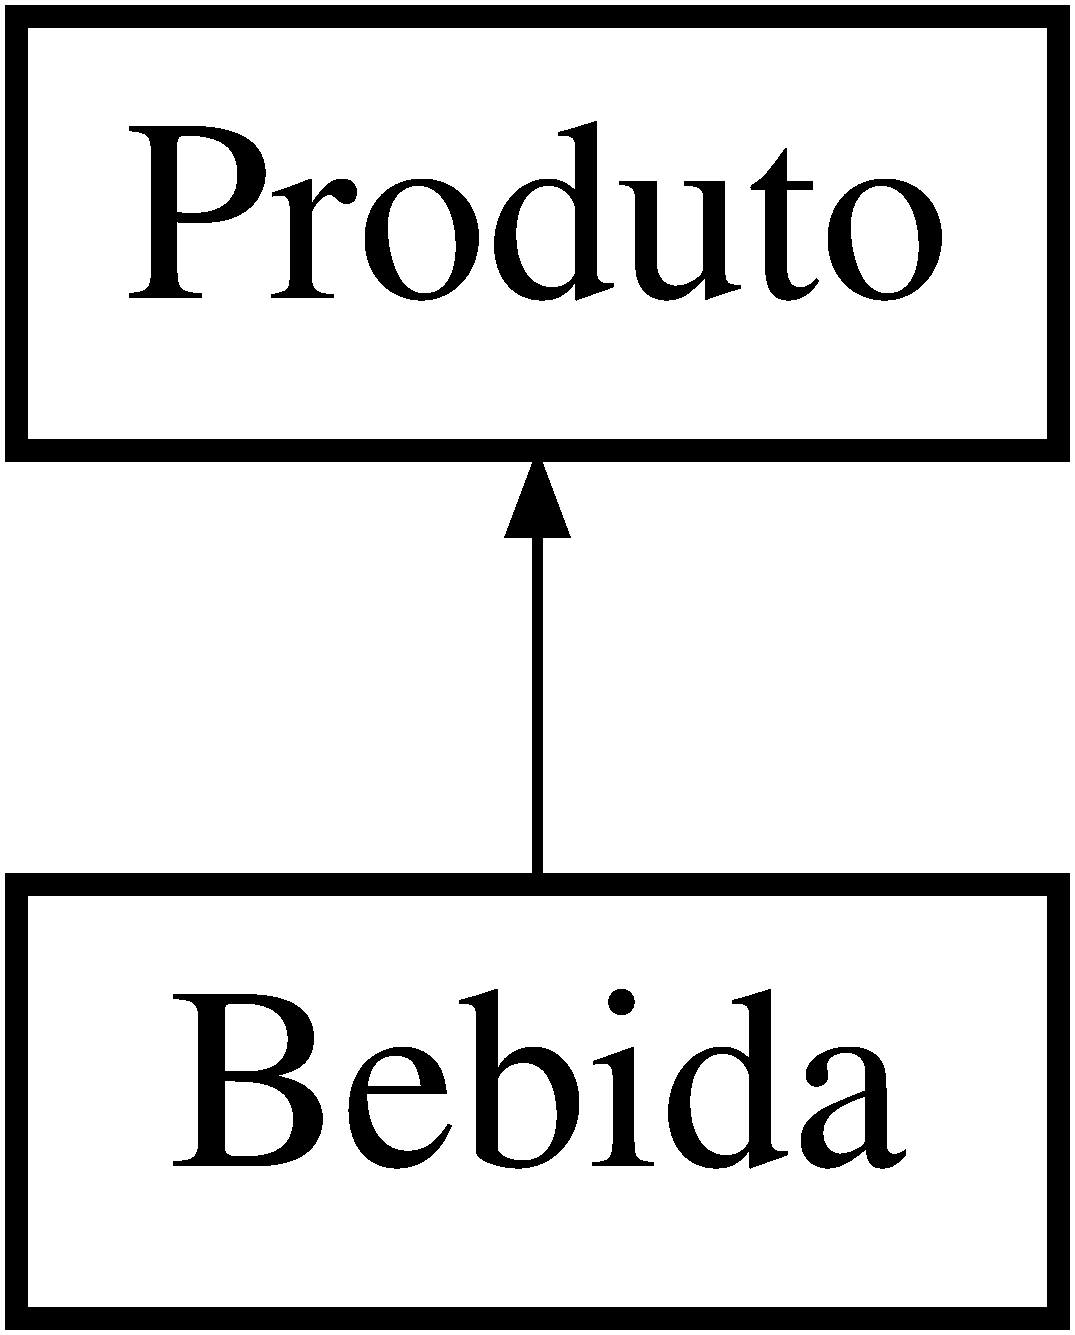
\includegraphics[height=2.000000cm]{classBebida}
\end{center}
\end{figure}
\subsection*{Public Member Functions}
\begin{DoxyCompactItemize}
\item 
\mbox{\Hypertarget{classBebida_a0c588567354f736594b8ee019f8d6ef4}\label{classBebida_a0c588567354f736594b8ee019f8d6ef4}} 
{\bfseries Bebida} (std\+::string \+\_\+codigo, std\+::string \+\_\+descricao, double \+\_\+preco, std\+::string \+\_\+teor)
\item 
\mbox{\Hypertarget{classBebida_ab24fcefd6e302a7fa61dc983472a3c83}\label{classBebida_ab24fcefd6e302a7fa61dc983472a3c83}} 
std\+::string {\bfseries get\+Teor} ()
\item 
\mbox{\Hypertarget{classBebida_a83400736aec54ffc0345cbbf260a157d}\label{classBebida_a83400736aec54ffc0345cbbf260a157d}} 
void {\bfseries set\+Teor} (std\+::string \+\_\+teor)
\end{DoxyCompactItemize}
\subsection*{Additional Inherited Members}


\subsection{Detailed Description}
Criação da classe \mbox{\hyperlink{classBebida}{Bebida}}. 


\begin{DoxyParams}{Parameters}
{\em Recebe} & os dados da classe mãe \mbox{\hyperlink{classProduto}{Produto}} e o teor Alcóolico da bebida em porcentagem \\
\hline
\end{DoxyParams}


The documentation for this class was generated from the following files\+:\begin{DoxyCompactItemize}
\item 
bebida.\+h\item 
bebida.\+cpp\end{DoxyCompactItemize}

\hypertarget{classFruta}{}\section{Fruta Class Reference}
\label{classFruta}\index{Fruta@{Fruta}}
Inheritance diagram for Fruta\+:\begin{figure}[H]
\begin{center}
\leavevmode
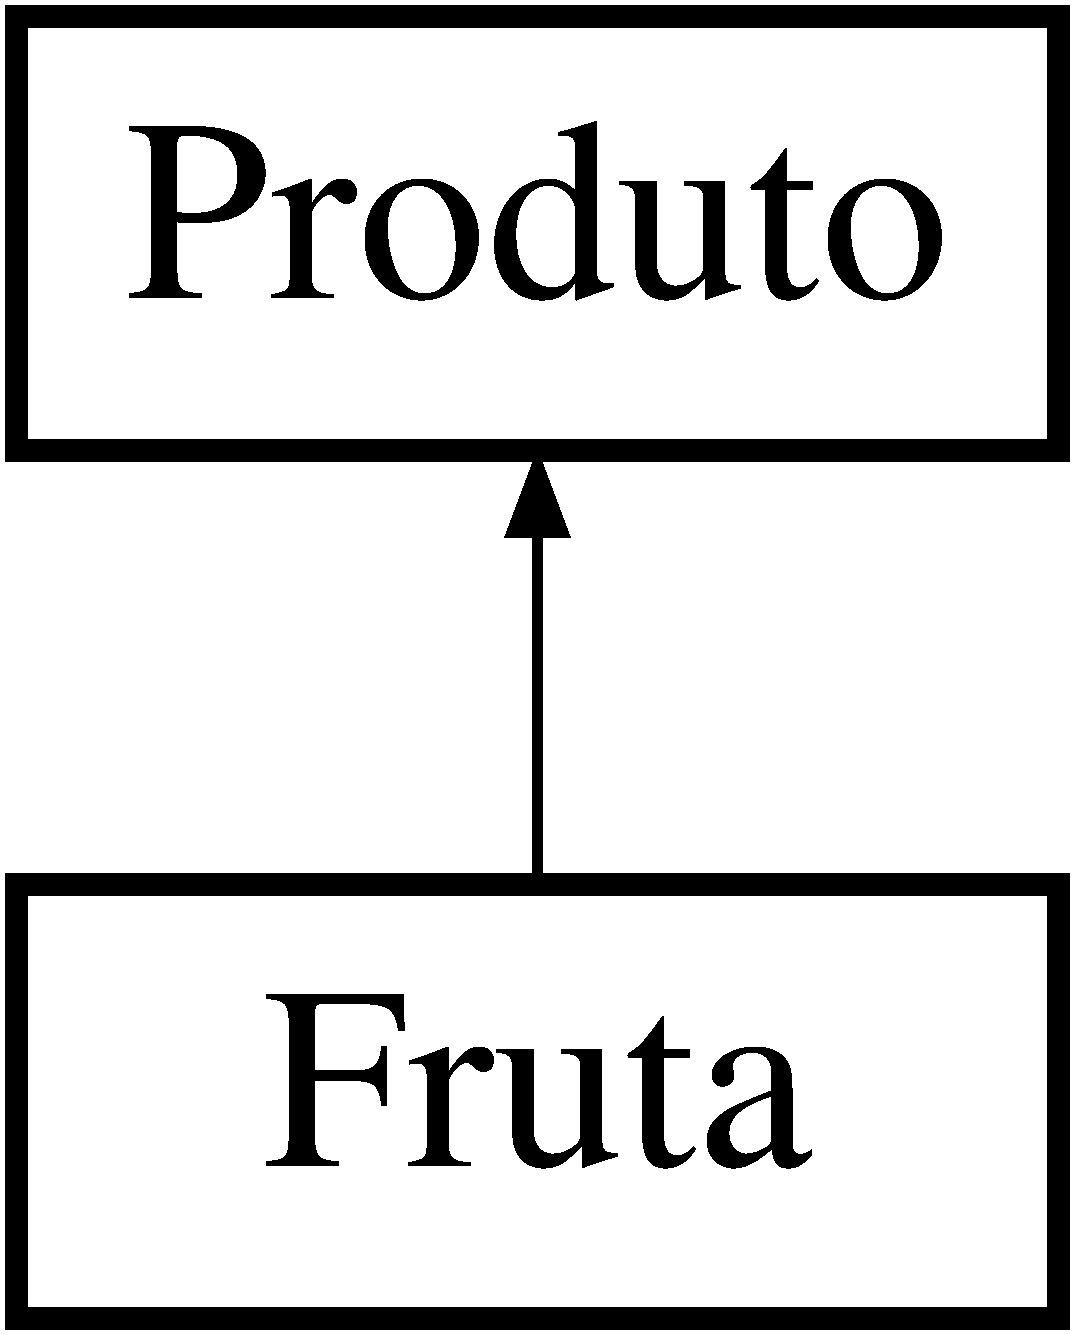
\includegraphics[height=2.000000cm]{classFruta}
\end{center}
\end{figure}
\subsection*{Public Member Functions}
\begin{DoxyCompactItemize}
\item 
\mbox{\Hypertarget{classFruta_a91cfd962d492f07be75bccea94e8cc5b}\label{classFruta_a91cfd962d492f07be75bccea94e8cc5b}} 
{\bfseries Fruta} (std\+::string \+\_\+codigo, std\+::string \+\_\+descricao, double \+\_\+preco, std\+::string \+\_\+data, short \+\_\+validade)
\item 
\mbox{\Hypertarget{classFruta_a89525ef74d892639b1a56dbf1c6ffe61}\label{classFruta_a89525ef74d892639b1a56dbf1c6ffe61}} 
std\+::string {\bfseries get\+Data\+Lote} ()
\item 
\mbox{\Hypertarget{classFruta_ab12db1faf3d5a0743ab461bc3315832e}\label{classFruta_ab12db1faf3d5a0743ab461bc3315832e}} 
short {\bfseries get\+Validade} ()
\item 
\mbox{\Hypertarget{classFruta_aa6cc01d8af01018e0a90b91e91884c13}\label{classFruta_aa6cc01d8af01018e0a90b91e91884c13}} 
void {\bfseries set\+Data\+Lote} (std\+::string \+\_\+data)
\item 
\mbox{\Hypertarget{classFruta_a779eb0307ab1f8e696d94f7420f43dbe}\label{classFruta_a779eb0307ab1f8e696d94f7420f43dbe}} 
void {\bfseries set\+Validade} (short \+\_\+validade)
\end{DoxyCompactItemize}
\subsection*{Additional Inherited Members}


The documentation for this class was generated from the following files\+:\begin{DoxyCompactItemize}
\item 
fruta.\+h\item 
fruta.\+cpp\end{DoxyCompactItemize}

\hypertarget{classProduto}{}\section{Produto Class Reference}
\label{classProduto}\index{Produto@{Produto}}


{\ttfamily \#include $<$produto.\+h$>$}

Inheritance diagram for Produto\+:\begin{figure}[H]
\begin{center}
\leavevmode
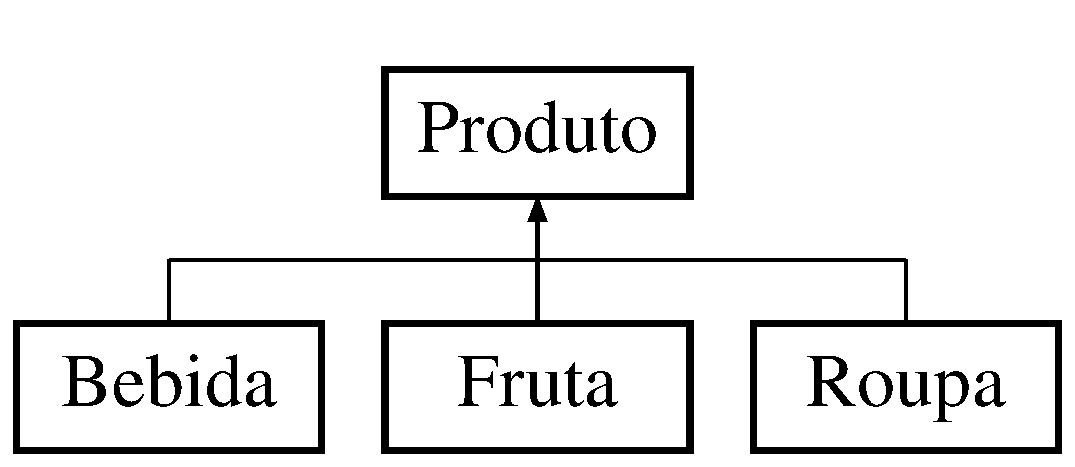
\includegraphics[height=2.000000cm]{classProduto}
\end{center}
\end{figure}
\subsection*{Public Member Functions}
\begin{DoxyCompactItemize}
\item 
\mbox{\Hypertarget{classProduto_a12dc783d4f1e016d1eefea0b3f83a6b0}\label{classProduto_a12dc783d4f1e016d1eefea0b3f83a6b0}} 
{\bfseries Produto} (std\+::string \+\_\+codigo, std\+::string \+\_\+descricao, double \+\_\+preco)
\item 
\mbox{\Hypertarget{classProduto_aa8e9057d5f0ac3d145333223cb513b3e}\label{classProduto_aa8e9057d5f0ac3d145333223cb513b3e}} 
std\+::string {\bfseries get\+Cod\+Barras} ()
\item 
\mbox{\Hypertarget{classProduto_ada2c72e139e09afa967aa06a4290d5f8}\label{classProduto_ada2c72e139e09afa967aa06a4290d5f8}} 
std\+::string {\bfseries get\+Descricao} ()
\item 
\mbox{\Hypertarget{classProduto_a53548783d7fad3ea6d5e000fa2227dcf}\label{classProduto_a53548783d7fad3ea6d5e000fa2227dcf}} 
double {\bfseries get\+Preco} ()
\item 
\mbox{\Hypertarget{classProduto_a8f8e7d58e53d3f175bc41b2481dbf477}\label{classProduto_a8f8e7d58e53d3f175bc41b2481dbf477}} 
void {\bfseries set\+Cod\+Barras} (std\+::string \+\_\+codigo)
\item 
\mbox{\Hypertarget{classProduto_a35b8ac377821ca2197becf75e1063509}\label{classProduto_a35b8ac377821ca2197becf75e1063509}} 
void {\bfseries set\+Descricao} (std\+::string \+\_\+descricao)
\item 
\mbox{\Hypertarget{classProduto_a207ec4b3438d376227ca3053a14669cf}\label{classProduto_a207ec4b3438d376227ca3053a14669cf}} 
void {\bfseries set\+Preco} (double \+\_\+preco)
\item 
double \mbox{\hyperlink{classProduto_a4b1186b555e78a10bc43dceceb2fde23}{operator+}} (\mbox{\hyperlink{classProduto}{Produto}} \&T)
\item 
\mbox{\Hypertarget{classProduto_a1d4f71551ca7db0485475e1492d2dab1}\label{classProduto_a1d4f71551ca7db0485475e1492d2dab1}} 
double {\bfseries operator-\/} (\mbox{\hyperlink{classProduto}{Produto}} \&T)
\item 
\mbox{\Hypertarget{classProduto_a847e805b411f2d893977662af67a2381}\label{classProduto_a847e805b411f2d893977662af67a2381}} 
bool {\bfseries operator==} (\mbox{\hyperlink{classProduto}{Produto}} \&T)
\end{DoxyCompactItemize}
\subsection*{Protected Attributes}
\begin{DoxyCompactItemize}
\item 
\mbox{\Hypertarget{classProduto_a2e772f6b851f2a2c7d7bc6853af7ca83}\label{classProduto_a2e772f6b851f2a2c7d7bc6853af7ca83}} 
std\+::string {\bfseries m\+\_\+cod\+\_\+barras}
\item 
\mbox{\Hypertarget{classProduto_aacf69c2cf01b6040138767a47c1e3f4b}\label{classProduto_aacf69c2cf01b6040138767a47c1e3f4b}} 
std\+::string {\bfseries m\+\_\+descricao}
\item 
\mbox{\Hypertarget{classProduto_af4f68aad97167802a1dca2b8ddb188eb}\label{classProduto_af4f68aad97167802a1dca2b8ddb188eb}} 
double {\bfseries m\+\_\+preco}
\end{DoxyCompactItemize}
\subsection*{Friends}
\begin{DoxyCompactItemize}
\item 
\mbox{\Hypertarget{classProduto_a75e56b3684b7859fc15d147b7d27f6b0}\label{classProduto_a75e56b3684b7859fc15d147b7d27f6b0}} 
std\+::ostream \& {\bfseries operator$<$$<$} (std\+::ostream \&o, \mbox{\hyperlink{classProduto}{Produto}} const \&t)
\end{DoxyCompactItemize}


\subsection{Detailed Description}
Se fez necessário ajustar de short para double a variável \+\_\+preco para compreender números decimais. 

\subsection{Member Function Documentation}
\mbox{\Hypertarget{classProduto_a4b1186b555e78a10bc43dceceb2fde23}\label{classProduto_a4b1186b555e78a10bc43dceceb2fde23}} 
\index{Produto@{Produto}!operator+@{operator+}}
\index{operator+@{operator+}!Produto@{Produto}}
\subsubsection{\texorpdfstring{operator+()}{operator+()}}
{\footnotesize\ttfamily double Produto\+::operator+ (\begin{DoxyParamCaption}\item[{\mbox{\hyperlink{classProduto}{Produto}} \&}]{T }\end{DoxyParamCaption})}

Criação dos métodos de sobrecarga\+: O método de soma e subtração retornam um valor float referente a soma ou subtração dos produtos. O método de igualdade compara os produtos e retorna verdadeiro em caso de igualdade, e falso caso contrário. 

The documentation for this class was generated from the following files\+:\begin{DoxyCompactItemize}
\item 
produto.\+h\item 
produto.\+cpp\end{DoxyCompactItemize}

\hypertarget{classRoupa}{}\section{Roupa Class Reference}
\label{classRoupa}\index{Roupa@{Roupa}}


Criação da classe \mbox{\hyperlink{classRoupa}{Roupa}}.  




{\ttfamily \#include $<$roupa.\+h$>$}

Inheritance diagram for Roupa\+:\begin{figure}[H]
\begin{center}
\leavevmode
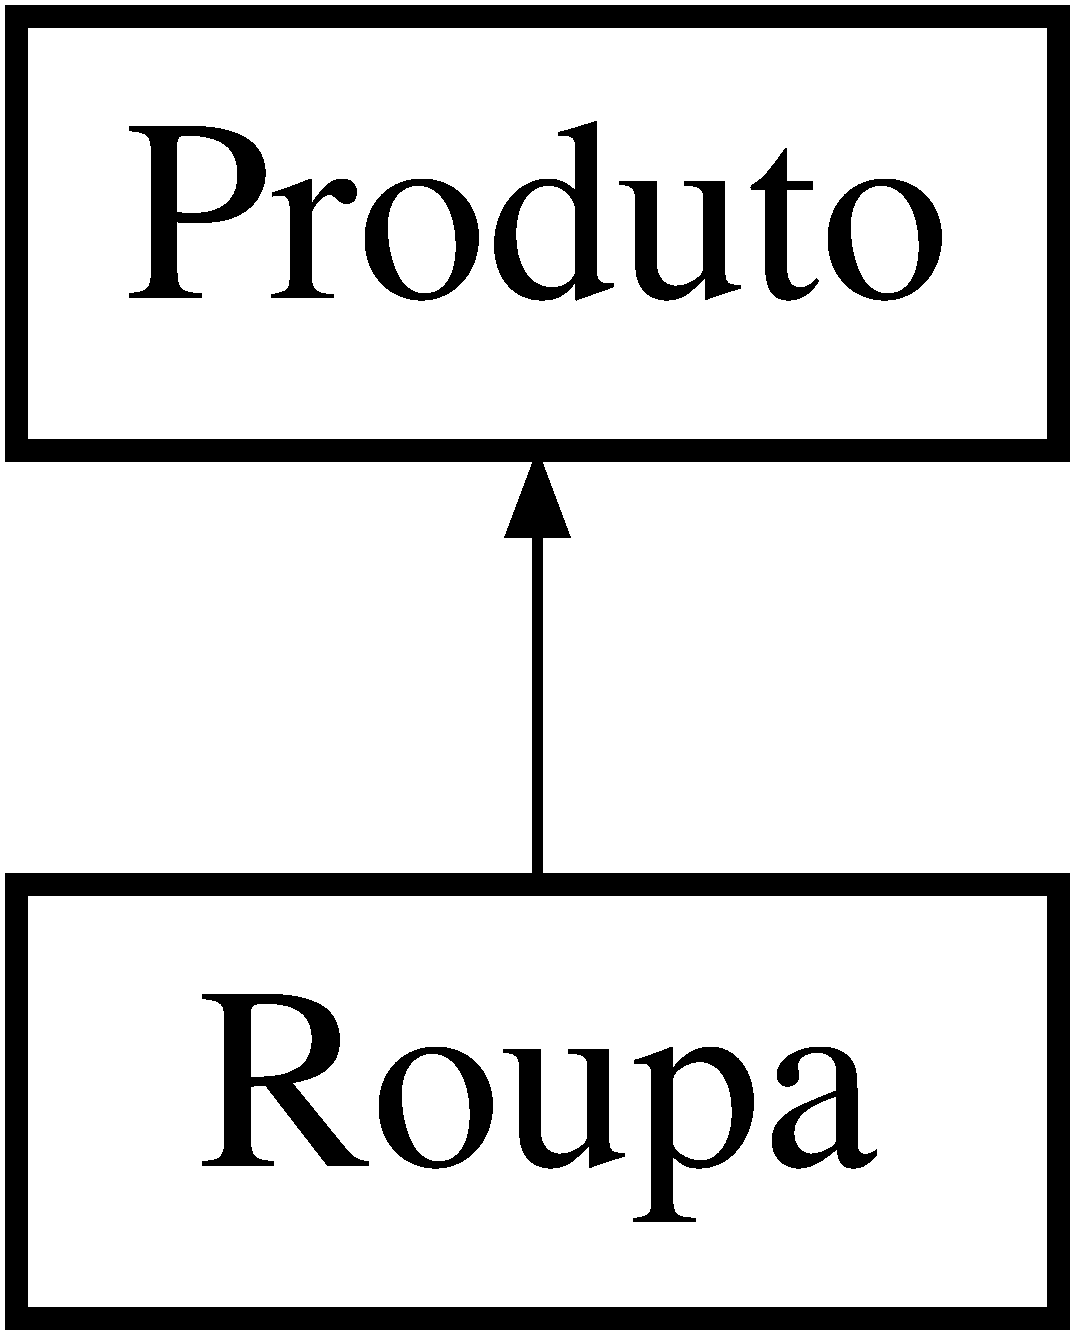
\includegraphics[height=2.000000cm]{classRoupa}
\end{center}
\end{figure}
\subsection*{Public Member Functions}
\begin{DoxyCompactItemize}
\item 
\mbox{\Hypertarget{classRoupa_a45c2f3690526dba425546f0b6d96a14d}\label{classRoupa_a45c2f3690526dba425546f0b6d96a14d}} 
{\bfseries Roupa} (std\+::string \+\_\+codigo, std\+::string \+\_\+descricao, double \+\_\+preco, std\+::string \+\_\+marca, std\+::string \+\_\+sexo, std\+::string \+\_\+tamanho)
\item 
\mbox{\Hypertarget{classRoupa_a627cb05c4d7401b97bae9902b6fcbff8}\label{classRoupa_a627cb05c4d7401b97bae9902b6fcbff8}} 
std\+::string {\bfseries get\+Marca} ()
\item 
\mbox{\Hypertarget{classRoupa_aef15096c554751e92045fc8acc257f18}\label{classRoupa_aef15096c554751e92045fc8acc257f18}} 
char {\bfseries get\+Validade} ()
\item 
\mbox{\Hypertarget{classRoupa_a6d3eb3fbbf40c0e12831ebebd3210ef0}\label{classRoupa_a6d3eb3fbbf40c0e12831ebebd3210ef0}} 
std\+::string {\bfseries get\+Tamanho} ()
\item 
\mbox{\Hypertarget{classRoupa_ac9fe45d8a8b73d28c15653ab8e8acdbb}\label{classRoupa_ac9fe45d8a8b73d28c15653ab8e8acdbb}} 
std\+::string {\bfseries get\+Sexo} ()
\item 
\mbox{\Hypertarget{classRoupa_a779827a9b55aa33229413fa441f45ab7}\label{classRoupa_a779827a9b55aa33229413fa441f45ab7}} 
void {\bfseries set\+Marca} (std\+::string \+\_\+marca)
\item 
\mbox{\Hypertarget{classRoupa_af34fb921628fbe9f26174699dd1748b2}\label{classRoupa_af34fb921628fbe9f26174699dd1748b2}} 
void {\bfseries set\+Sexo} (std\+::string \+\_\+sexo)
\item 
\mbox{\Hypertarget{classRoupa_ab5541947bc4fde1925422eab8cc6b190}\label{classRoupa_ab5541947bc4fde1925422eab8cc6b190}} 
void {\bfseries set\+Tamanho} (std\+::string \+\_\+tamanho)
\end{DoxyCompactItemize}
\subsection*{Additional Inherited Members}


\subsection{Detailed Description}
Criação da classe \mbox{\hyperlink{classRoupa}{Roupa}}. 


\begin{DoxyParams}{Parameters}
{\em Recebe} & os dados da classe mãe \mbox{\hyperlink{classProduto}{Produto}}, o sexo sendo (M ou F), a marca, e o tamanho(\+P\+P,\+P,\+M,\+G ou G\+G) \\
\hline
\end{DoxyParams}


The documentation for this class was generated from the following files\+:\begin{DoxyCompactItemize}
\item 
roupa.\+h\item 
roupa.\+cpp\end{DoxyCompactItemize}

%--- End generated contents ---

% Index
\backmatter
\newpage
\phantomsection
\clearemptydoublepage
\addcontentsline{toc}{chapter}{\indexname}
\printindex

\end{document}
